%
% Berechnung der Zahl der Spanning Trees eines Graphen mit Hilfe
% der Determinante, Anwendung zu Kapitel 2, Determinanten
%
Kirchhoff hat nicht nur gezeigt, wie die Gleichungen f"ur Spannungen
und Str"ome in einem Widerstandsnetzwerk aufzustellen sind, dies
haben wir in \ref{appkirchhoff} dargestellt, er hat
auch einiges "uber die L"osungen herausgefunden.
Ausserdem haben sich seine Ideen als fruchtbar in der Netzwerktheorie
erwiesen, als Beispiel zeigen wir, wie man mit Determinanten die
Zahl der Spannb"aume in einem Netzwerk berechnen kann.

\subsection{L"osung der Kirchhoff-Gleichungen}
Gehen wir wieder aus von einem Netzwerk wie in
Abbildung~\ref{netzwerk-numeriert}, wir verwenden die selben 
Bezeichnungen wie in Abschnitt \ref{appkirchhoff}.
Die Gleichungen nach Kirchhoff sind dann
\begin{align*}
Z^tRI&=Z^te \tag{Maschengleichungen}\\
\partial I&=0 \tag{Knotengleichungen}
\end{align*}
Wir wissen bereits, dass ein Netzwerk mit $n$ Kanten und $m$
Knoten $n-m+1$ linear unabh"angige Maschengleichungen und
$m-1$ linear unabh"angige Knotengleichungen hat, mit denen man
die $n$ Str"ome $I$ bestimmen kann.

Kirchhoff hat seine Gleichungen so geschrieben:
\begin{center}
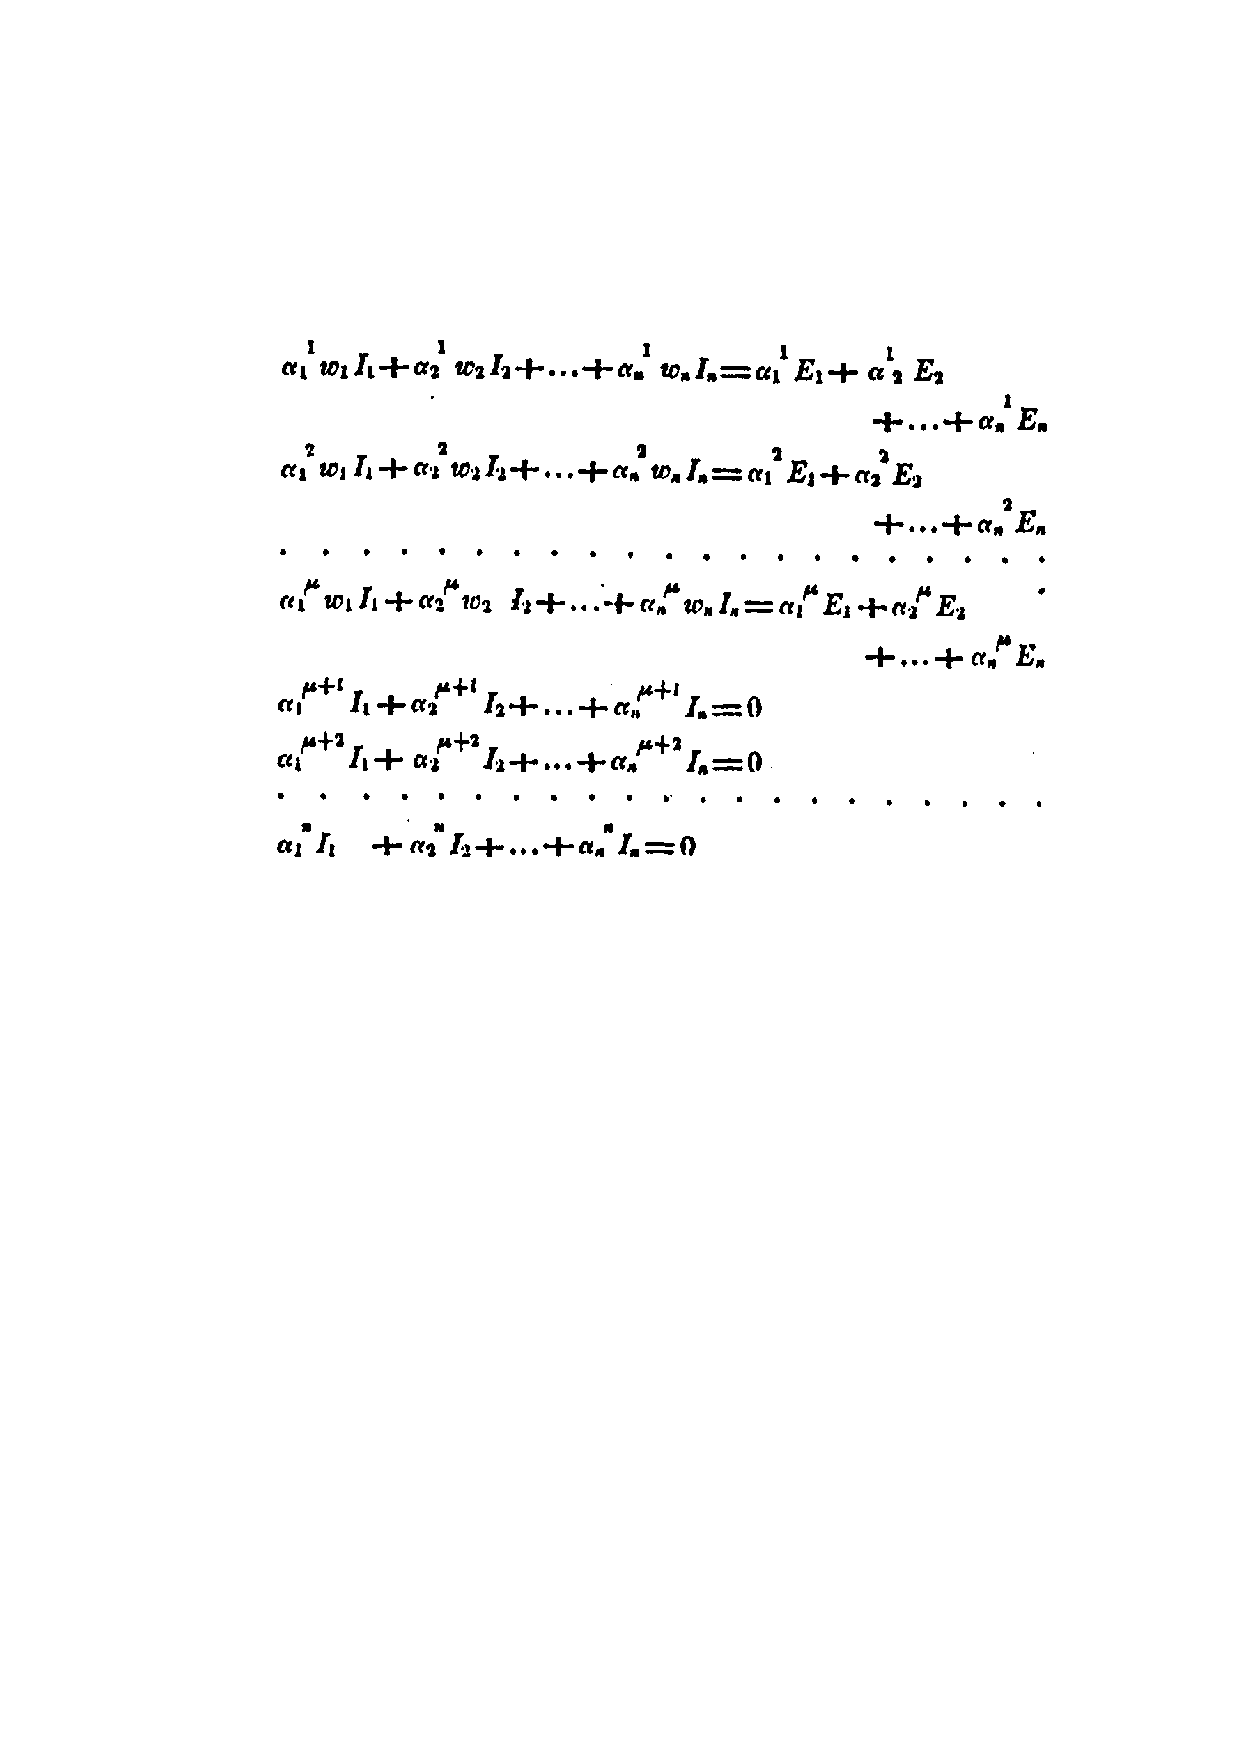
\includegraphics[width=0.8\hsize]{graphics/kh3}
\end{center}
In unserer modernen Schreibweise mit den Notationen von
Abschnitt~\ref{appkirchhoff} sind sie
\[
\begin{linsys}{5}
z_{11}R_1I_1&+&z_{21}R_2I_2&+&\dots &+&z_{n1}R_nI_n&=&z_{11}e_1&+&z_{21}e_2+\dots+z_{n1}e_n=b_1\\
      \vdots& &\vdots      & &\ddots& &\vdots      & &         & & \\
z_{1s}R_1I_1&+&z_{2s}R_2I_2&+&\dots &+&z_{ns}R_nI_n&=&z_{1s}e_1&+&z_{2s}e_2+\dots+z_{ns}e_n=b_s\\
   \partial_{11}I_1&+&   \partial_{12}I_2&+&\dots &+&   \partial_{1n}I_n&=&0&&\\
             \vdots& &   \vdots          & &\ddots& &             \vdots& &\vdots&&\\
\partial_{m-1,1}I_1&+&\partial_{m-1,2}I_2&+&\dots &+&\partial_{m-1,n}I_n&=&0&&\\
\end{linsys}
\]
Die Koeffizienten $z_{ij}$ sind die Matrixelemente der Zyklen-Matrix $Z$.
Kirchhoff versucht dann, die Str"ome $I_i$ mit der Cramerschen 
Regel, also mit Hilfe von Determinanten zu bestimmen.
Dazu muss die Determinante der Koeffizienten-Matrix bestimmt werden.
Der Nenner ist
\begin{equation}
N=\left|\;\begin{matrix}
z_{11}R_1       &z_{21}R_2       &\dots &z_{n1}R_n       \\
\vdots          &\vdots          &\ddots&\vdots          \\
z_{1s}R_1       &z_{2s}R_2       &\dots &z_{ns}R_n       \\
\partial_{11}   &\partial_{12}   &\dots &\partial_{1n}   \\
\vdots          &\vdots          &\ddots&\vdots          \\
\partial_{m-1,1}&\partial_{m-1,2}&\dots &\partial_{m-1,n}
\end{matrix}\;\right|
=
\left|\;
\begin{tabular}{>{$}c<{$}>{$}c<{$}>{$}c<{$}}
&          &\\
&Z^tR      &\\
&          &\\
%\hline
%&          &\\
&\partial_-&\\
&          &
\end{tabular}
\;\right|.
\label{Ndenominator}
\end{equation}
Dabei meinen wir mit $\partial_-$ die Matrix, die aus $\partial$
entsteht, indem man die letzte Zeile wegl"asst.

Sowohl die $z_{ij}$ wie auch die $\partial_{ij}$ sind aus $\{-1,0,+1\}$.
Bei der Entwicklung der Determinante entstehen also jeweils Terme
mit genau $s$ Faktoren $R_i$ und einem Vorzeichen.
Beispielsweise entsteht der Term mit $R_1R_2\dots R_s$ durch
Auswahl von Elementen aus $s\times s$-Block in der linken oberen
Ecke, und verbleibenden Elementen aus dem $(m-1)\times (m-1)$-Block
aus der rechten unteren Ecke, er ist
\[
R_1R_2\dots R_s
\left|\;
\begin{matrix}
z_{11}       &z_{21}       &\dots &z_{s1}       \\
\vdots       &\vdots       &\ddots&\vdots       \\
z_{1s}       &z_{2s}       &\dots &z_{ss}       
\end{matrix}
\;\right|
\cdot
\left|\;
\begin{matrix}
\partial_{1,s+1}   &\partial_{1,s+2}   &\dots &\partial_{1n}   \\
\vdots             &\vdots             &\ddots&\vdots          \\
\partial_{m-1,s+1} &\partial_{m-1,s+2} &\dots &\partial_{m-1,n}
\end{matrix}
\;\right|
\]
W"ahlt man beliebige Indizes $i_1,i_2,\dots,i_s$, und sind $j_1,\dots,j_{m-1}$
die "ubrigen Indizes, dann ist der
Term mit $R_{i_1}R_{i_2}\dots R_{i_s}$ entsprechend:
\[
\sigma(i_1,\dots,i_s)
R_{i_1}R_{i_2}\dots R_{i_s}
\left|\;
\begin{matrix}
z_{i_1,1}    &\dots &z_{i_s,1}\\
\vdots       &\ddots&\vdots   \\
z_{i_1,s}    &\dots &z_{i_s,s}       
\end{matrix}
\;\right|
\cdot
\left|\;
\begin{matrix}
\partial_{1,j_1}   &\dots &\partial_{1j_{m-1}}   \\
\vdots             &\ddots&\vdots          \\
\partial_{m-1,j_1} &\dots &\partial_{m-1,j_{m-1}}
\end{matrix}
\;\right|
\]
Darin ist $\sigma(i_1,\dots,i_n)$ ein Vorzeichenfaktor, der
daher r"uhrt, dass man die Spalten $i_1,\dots,i_s$ zun"achst
mit Spalten-Vertauschungen in Positionen $1,\dots,s$ bringen
will.

Zur Ermittlung des Stromes $I_l$ muss in dieser Determinante die
Spalte $l$ mit durch die rechte Seite ersetzt werden. Dadurch
entstehen bei der Entwicklung der Determinanten "ahnliche Terme,
allerdings kommt genau ein $R$ weniger vor.

Es scheint auf den ersten Blick ziemlich aussichtslos, diese
Determinanten zu berechnen, nur gerade die Struktur von Z"ahler
und Nenner kann man ermitteln. Schreiben wir $B_l$ f"ur den 
Z"ahler, der zur Berechnung von $I_l$ ben"otigt wird, dann ist
\begin{align*}
B_l&=\sum_{i_1,\dots,i_{s-1}}A^l_{i_1,\dots,i_{s-1}}R_{i_1}\dots R_{i_{s-1}}\\
N&=\sum_{i_1,\dots,i_s}a_{i_1,\dots,i_s}R_{i_1}\dots R_{i_s}\\
I_l&=\frac{B_l}{N}
\end{align*}
mit noch zu bestimmenden Koeffizienten $A_{i_1,\dots,i_{s-1}}^l$
und $a_{i_1,\dots,i_s}$.

\subsubsection{Kirchhoffs Idee}
Die Berechnung der Koeffizienten wird m"oglich dank einer brillanten
Idee Kirchhoffs. L"asst man einzelne Widerst"ande im Netzwerk gegen
$\infty$ gehen, werden sich die Str"ome auf neue Werte $I_{l,\infty}$
einstellen. Anderseits k"onnte man diese Widerst"ande auch gleich entfernen.
Man erhielte dann ein neues Netzwerk und neue Koeffizienten
\[
A_{i_1,\dots,i_{s'-1}}^{\prime l}
\quad
\text{und}
\quad
a_{i_1,\dots,i_{s'}}
\]
Diese Koeffizienten gestatten die Str"ome $I'_l$ des modifizierten Netzwerks
zu berechnen. Nat"urlich muss $I_{l,\infty}=I'_l$ gelten.

Wenden wir diese Operation auf die ersten $s-1$ Dr"ahte des Netzwerkes
an. Die Widerst"ande $R_1,\dots,R_{s-1}$ werden also beliebig gross gemacht.
Sowohl im Z"ahler wie auch im Nenner von $I_l$ kommen Produkte von diesen
Widerst"anden vor. Am st"arksten wachsen werden aber die Terme, die
alle $s-1$ Widerst"ande enthalten. K"urzen wir den ganzen Bruch durch
$R_1\dots R_{s-1}$, dann bleibt im Z"ahler
\[
\frac{B_l}{R_1\dots R_{s-1}}=
A_{1,\dots,s-1}^l+r_l(R_1,\dots,R_n)
\]
wobei in jedem Term des Restes $r_l(R_1,\dots,R_n)$ mindestens einer
der Widerst"ande $R_1,\dots,R_{s-1}$ im Nenner vorkommt, der Rest
strebt also gegen $0$, wenn man die Widerst"ande gross macht.
Im Nenner bleiben in "ahnlicher Weise die Terme
\[
\frac{N}{R_1\dots R_{s-1}}=
a_{1,\dots,s-1,s}R_s+a_{1,\dots,s-1,s+1}R_{s+1}+\dots+a_{1,\dots,s-1,n}R_n
+q(R_1,\dots,R_n)
\]
stehen, wobei der Rest $q(R_1,\dots,R_n)$ f"ur wachsende Widerst"ande
gegen $0$ strebt. Folglich sind die Grenzstr"ome im Netzwerk mit den
gegen unendlich strebenden Widerst"anden
\begin{equation}
I_{l,\infty}=
\frac{A_{1,\dots,s-1}^l}{a_{1,\dots,s-1,s}R_s+a_{1,\dots,s-1,s+1}R_{s+1}+\dots+a_{1,\dots,s-1,n}R_n}.
\label{Iinfinity}
\end{equation}
Wenn $l$ einer der Widerst"ande ist, den man gegen $\infty$ hat gehen lassen,
dann ist $I_{l,\infty}=0$ und nach $I'_l$ zu fragen hat keinen Sinn, diese
Kante gibt es im modifizierten Netzwerk nicht mehr. F"ur alle anderen 
Kanten muss $I_{l,\infty}=I_l'$ gelten:
\begin{equation}
I_{l,\infty}=
\begin{cases}
0&\quad l< s\\
I'_l&\quad\text{sonst}.
\end{cases}
\label{Iequations}
\end{equation}
Damit haben wir eine ganze Menge Gleichungen, die erf"ullt sein
m"ussen, und es besteht die Hoffnung, dass sich daraus die Koeffizienten
bestimmen lassen.

\subsubsection{Ein einzelner Zyklus}
Wenn nach der Entfernung von $s-1$ Dr"ahten nur noch ein einzelner
Zyklus "ubrig bleibt, dann l"asst sich die L"osung sofort angeben.
Innerhalb des Zyklus muss der Strom immer gleich sein, und alle
Kanten ausserhalb des Zyklus haben Strom $0$. Sind $l_1,\dots,l_k$
die Kanten des Zyklus, dann ist die einzige verbleibende Kirchhoffsche
Gleichung:
\begin{align}
R_{l_1}I_{l_1}'+R_{l_2}I_{l_2}'+R_{l_k}I_{l_k}'&=e_{l_1}+e_{l_1}+\dots+e_{l_k}
\notag
\\
I_{l_1}'=I_{l_2}'=\dots=I_{l_k}'&=\frac{e_{l_1}+e_{l_1}+\dots+e_{l_k}}{R_{l_1}+R_{l_2}+\dots+R_{l_k}}.
\label{singlecycleprime}
\end{align}
Es sieht also so aus, als h"atten wir den Koeffizienten bereits
bestimmt, (\ref{Iinfinity}) sieht doch sehr "ahnlich wie
(\ref{singlecycleprime}) aus. Leider reicht das nicht ganz, Der Bruch
$I_{l,\infty}$ k"onnte gegen"uber $I'_l$ auch erweitert worden sein.

Doch mindestens k"onnen wir ablesen, dass $a_{1,\dots,s-1,i}=0$ ist,
wenn $i$ nicht zum Zyklus $l_1,\dots,l_k$ geh"ort. Im Nenner von
$I_{l,\infty}$ k"onnen also nur Terme vorkommen, deren letzter Index
zum einzigen verbleibenden Zyklus geh"ort.
Ausserdem m"ussen diese Koeffizienten alle gleich sein:
\begin{equation}
a_{1,\dots,s-1,l_1}=a_{1,\dots,s-1,l_2}=\dots= a_{1,\dots,s-1,l_k}
\label{cyclecoefficients}
\end{equation}
\begin{hilfssatz}
\label{gleichekoef-n-1}
Wenn das Entfernen der Kanten $i_1,\dots,i_{s-1}$ genau einen
Zyklus "ubrig l"asst, dann sind alle Koeffizienten
$a_{i_1,\dots,i_{s-1},l}$ gleich, wenn $l$ eine Kante des letzten
verbleibenden Zyklus ist.
\end{hilfssatz}
Damit ergibt sich jetzt der Plan f"ur die weitere Untersuchung:
\begin{compactenum}
\item In dem Fall, dass nach Entfernen der ersten $s-1$ Kanten mehr als $1$
Zyklus "ubrig bleibt, m"ussen wir zeigen, dass dann $R_1\dots R_{s-1}$
in Z"ahler und Nenner gar nicht vorkommt, dass die Koeffizienten
$A_{1,\dots,s-1}^l$ und $a_{1,\dots,s-1,i}$ alle verschwinden.
\item Nicht nur die Koeffizienten zu einem einzelnen Zyklus
wie in (\ref{cyclecoefficients}) sind untereinander gleich, es sind
sogar alle nicht verschwindenden Koeffizienten gleich.
\end{compactenum}

\subsubsection{Mehr als ein Zyklus}
Nehmen wir jetzt an, dass nach dem Entfernen der ersten $s-1$ Kanten
$s'>1$ Zyklen "ubrig bleiben.
Die Gleichungen (\ref{Iequations}) k"onnen auf verschiedene Arten
zustande kommen.
\begin{compactenum}
\item Der Bruch $I_l'$ kann durch einen gemeinsamen Faktor
$R_{j_1}\dots R_{j_{s'-1}}$ gek"urzt werden.

In diesem Fall gibt es also einen gemeinsamen Faktor
$R_{j_1}\dots R_{j_{s'-1}}$ in Z"ahler und Nenner von $I_l'$.
Da nur Widerst"ande in den Nenner
eingehen, die in einem Zyklus vorkommen, gibt es einen Widerstand
$R_x$ welcher sowohl in $R_{j_1}\dots R_{j_{s'-1}}$ als auch in
einem Zyklus vorkommt.
K"urzt man jetzt $R_{j_1}\dots R_{j_{s'-1}}$, entstehen in Z"ahler und
Nenner Ausdr"ucke, in denen $R_x$ nicht mehr vorkommt. 
Insbesondere h"angt $I_x'$ nicht mehr von $R_x$ ab, auch f"ur sehr grosses
$R_x$ nicht. Daher muss $I_x'=0$ sein, f"ur beliebige Werte der Widerst"ande
und elektromotorischen Kr"afte.
Das kann aber nicht sein, denn wenn man so viele weitere Widerst"ande 
beliebig gross macht, dass nur noch eine Zyklus verbleibt, der $R_x$
enth"alt, dann kann man durch Anpassen der elektromotorischen Kr"afte
einen Strom in diesem Zyklus zum fliessen bringen. Dieser Fall kann
also nicht eintreten.
\item Der Z"ahler in $I_{l,\infty}$ und $I_l'$ verschwindet.
Dieser Fall erm"oglicht uns allerdings nicht, weiter Aussagen
"uber die $a$-Koeffizienten zu machen.
\item Z"ahler und Nenner in $I_{l,\infty}$ verschwinden.
Da dieser Fall die einzige verbleibende M"oglichkeit ist, m"ussen
also alle Koeffizienten $a_{1,\dots,s,i}$ und $A^l_{1,\dots,s-1}$
verschwinden, wenn durch Entfernung der ersten $s-1$ Kanten mehr als
ein Zyklus verbleibt.
\end{compactenum}
Als Resultat haben wir, dass nur Koeffizienten $a_{i_1,\dots,i_{s-1}}$
und $A_{i_1,\dots,i_{s-1}}^l$ von $0$ verschieden sein k"onnen, 
wenn die Entfernung der Kanten $i_1,\dots,i_{s-1}$ genau einen
Zyklus "ubrig l"asst.

\begin{hilfssatz}
Die Koeffizienten $a_{i_1,\dots,i_s}$ sind nur dann von $0$ verschieden,
wenn durch Entfernen der Kanten $i_1,\dots,i_s$ alle Zyklen zerst"ort
werden.
\end{hilfssatz}

\begin{proof}[Beweis]
Wenn $i_1,\dots,i_s$ alle Zyklen zerst"ort, dann l"asst
$i_1,\dots,i_{s-1}$ genau einen Zyklus "ubrig, und $i_s$ 
geh"ort zu diesem verbleibenden Zyklus. Dann ist nach dem
eben gezeigten $a_{i_1,\dots,i_s}\ne 0$.
\end{proof}

\subsubsection{Gleichheit der Koeffizienten}
Bis jetzt wissen wir, dass alle Terme $R_{i_1}\dots R_{i_{s-1}}R_j$
im Nenner von $I_{l,\infty}$ den gleichen Koeffizienten haben,
wenn nach Entfernung der Kanten $i_1,\dots,i_{s-1}$ genau ein
Zyklus verbleibt, und $j$ in diesem Zyklus liegt. Wir wollen jetzt
einsehen, dass "uberhaupt alle Koeffizienten im Nenner gleich sind.

\begin{hilfssatz}
\label{gleichekoef-induktionsschritt}
Wenn die $a$-Koeffizienten gleich sind,
wenn mindestens $\nu$ Kanten "ubereinstimmen,
dann sind die Koeffizienten auch gleich,
wenn nur die ersten $\nu-1$ Kanten "ubereinstimmen.
\end{hilfssatz}

\begin{proof}[Beweis]
Seien
$i_1,\dots,i_\nu,i_{\nu+1},\dots,i_s$
und
$i_1,\dots,i_{\nu},i'_{\nu+1},\dots,i_s'$
Kantenmengen,
durch deren
Entfernung alle Zyklen zerst"ort werden,
und die in den ersten $\nu$ Kanten "ubereinstimmen.
Dann wird durch $i_\nu'$ ein Zyklus zerst"ort, der auch von einem
der Indizes $i_{k}$ mit $k\ge\nu$ zerst"ort wird. Ohne Einschr"ankung
der Allgemeinheit k"onnen wir annehmen, dass $i_{\nu}$ diese Kante ist.

Dann gibt es ausserdem Kanten $i_{\nu+1}'',\dots,i_s''$, durch deren
Entfernung die verbleibenden $s-\nu$ Zyklen zerst"ort werden. Die Kantenmengen
\begin{align*}
&i_1,\dots,i_{\nu-1},i_{\nu},i_{\nu+1},\dots,i_s\\
&i_1,\dots,i_{\nu-1},i_{\nu},i_{\nu+1}'',\dots,i_s''\\
&i_1,\dots,i_{\nu-1},i_{\nu}',i_{\nu+1}'',\dots,i_s''\\
&i_1,\dots,i_{\nu-1},i_{\nu}',i_{\nu+1}',\dots,i_s'
\end{align*}
zerst"oren alle Zyklen, und haben von Zeile zu Zeile mindestens
$\nu$ gemeinsame Kanten (im mittleren Schritt sogar $s-1$
gemeinsame Kanten). Daher sind die Koeffizienten gleich:
\[
a_{i_1,\dots,i_{\nu-1},i_{\nu},i_{\nu+1},\dots,i_s}
=
a_{i_1,\dots,i_{\nu-1},i_{\nu},i_{\nu+1}'',\dots,i_s''}
=
a_{i_1,\dots,i_{\nu-1},i_{\nu}',i_{\nu+1}'',\dots,i_s''}
=
a_{i_1,\dots,i_{\nu-1},i_{\nu}',i_{\nu+1}',\dots,i_s'},
\]
was die Behauptung beweist.
\end{proof}

\begin{satz}
Wenn $i_1,\dots,i_s$ und $j_1,\dots,j_s$ alle Zyklen zerst"oren,
dann ist 
\[
a_{i_1,\dots,i_s}=a_{j_1,\dots,j_s}.
\]
\end{satz}

\begin{proof}[Beweis]
Nach Hilfssatz~\ref{gleichekoef-n-1} gilt die Behauptung, wenn die Kantenmengen
$n-1$ gemeinsame Kanten haben.
Nach Hilfssatz~\ref{gleichekoef-induktionsschritt} folgt Gleichheit der
Koeffizienten auch, wenn weniger Kanten "ubereinstimmen.
\end{proof}

\subsubsection{Die L"osung der Kirchhoff-Gleichungen}
Da wir jetzt alle Nenner kennen, k"onnen wir auch die L"osung
der Gleichung unmittelbar angeben.
Zun"achst wissen wir, dass alle Koeffizienten der Terme
$R_{i_1}\dots R_{i_s}$ alle identisch sind, wenn $i_1,\dots,i_s$
alle Zyklen des Netzwerks zerst"ort,
\[
N =\sum_{i_1,\dots,i_s}R_{i_1}\dots R_{i_s}.
\]
Die Koeffizienten im Z"ahler kann man durch Vergleich
mit (\ref{singlecycleprime}) bekommen. Wenn nach Entfernung
von $i_1,\dots,i_{s-1}$ noch ein Zyklus $l_1,\dots,l_k$ bleibt, dann
ist
\[
A_{i_1,\dots,i_{s-1}}^l=\begin{cases}
e_{l_1}+\dots+e_{l_k}&\quad l\in\{l_1,\dots,l_k\}\\
0&\quad \text{sonst.}
\end{cases}
\]
Damit lassen sich die Kirchhoffschen Gleichungen dadurch l"osen,
dass man alle Kantenmengen untersucht, die alle Zyklen zerst"oren.

\subsection{Spannb"aume}
\index{Spannbaum}
Ein Spannbaum eines Netzwerks ist eine zyklenfreie Teilmenge der Kanten,
welche alle Knoten miteinander verbindet.
Ein Spannbaum ist also genau das, was "ubrig bleibt, wenn man aus dem
Netzwerk $s$ Kanten entfernt hat, so dass keine Zyklen mehr "ubrig bleiben.
Setzt man alle Widerst"ande des Netzwerkes auf Wert $1$, also
$R_1=\dots=R_n=1$ oder $R=E$,
dann ist der Nenner der L"osung der Kirchhoff-Gleichungen
genau die Zahl der Spannb"aume des Netzwerkes. Die Kirchhoff-Gleichungen
k"onnten also eine M"oglichkeit liefern, die Zahl der Spannb"aume
zu z"ahlen. 
Leider erinnert uns die Formel (\ref{Ndenominator}) auch daran, dass  
wir den Nenner nur bis auf einen Faktor bestimmt haben. In der
Tat k"onnen wir die Zyklen in $Z^t$ mit beliebigen Faktoren
multiplizieren. Um die Zyklen zu z"ahlen, brauchen wir also
ein Verfahren, welches $Z$ gar nicht braucht.

Die Matrix auf der rechten Seite von (\ref{Ndenominator}) gibt uns den
Schl"ussel. Multiplizieren wir sie mit der Transponierten bekommen
wir
\begin{equation}
\begin{pmatrix}
Z^t\\
\partial_-
\end{pmatrix}
\begin{pmatrix}
Z&\partial_-^t
\end{pmatrix}
=\begin{pmatrix}
Z^tZ&Z^t\partial_-^t\\
\partial_-Z&\partial_-\partial_-^t
\end{pmatrix}
\end{equation}
Die Bl"ocke ausserhalb der Diagonalen verschwinden, $\partial_-Z=0$
und $Z^t\partial_-^t=(\partial_-Z)^t=0$, weil die Spalten von $Z$ Zyklen sind.
"Ubrig bleibt also die Determinante
\begin{equation}
\det
\begin{pmatrix}
Z^tZ&0\\
0&\partial_-\partial_-^t
\end{pmatrix}
=\det(Z^tZ)\det(\partial_-\partial_-^t)
\end{equation}
Der erste Term auf der rechten Seite enth"alt offenbar alles, was von
der speziellen Wahl der Zyklen abh"angt. Nur der zweite Teil ist
unabh"angig, von der Wahl der Zyklen. $\partial_-\partial_-^t$ ist derjenige
Teil des Laplace-Operators des Netzwerk, den man durch Weglassen der
letzten Zeile und Spalte bekommt.

Aus Kirchhoffs Untersuchung wissen
wir, dass es nicht darauf ankommt, welche Zeile man in $\partial$ 
wegl"asst, um $\partial_-$ zu bilden. Alle so gebildeten
Matrizen m"ussten also die selbe Determinante haben.

\index{Matrix-Baum-Satz}
\begin{satz}[Matrix-Baum-Satz von Kirchhoff] Die Zahl $\tau(G)$
\label{matrixtreetheorem}
der Spannb"aume eines
Netzwerks $G$ ist gegeben durch den Wert der Kofaktoren des Laplace-Operators
$\Delta_G$.
Alle Kofaktoren sind gleich.
\end{satz}
Wir teilen den Beweis in mehrere Schritte auf, die f"ur sich genommen
auch interessante Resultate sein k"onnen. 

\begin{hilfssatz}
Ist in einer $n\times n$-Matrix $A$ die Summe jeder Zeile und jeder
Spalte $0$, dann sind alle Kofaktoren von $A$ gleich.
\end{hilfssatz}
\begin{proof}[Beweis]
Wir zeigen, dass ein beliebiger Kofaktor
$\operatorname{cof}(A)_{ij}=\operatorname{cof}(A_{nn})$ ist.
wir schreiben wieder $a_k$ f"ur den $k$-ten Spaltenvektor von $A$.

Weil die Zeilen- und Spaltensumme immer $0$ ist, sind sowohl die
Zeilen wie auch die Spalten linear abh"angig. Insbesondere kann die Spalte
$n$ als Linearkombination der anderen Spalten geschrieben werden:
\[
a_n=-a_1-a_2-\dots-a_{n-1}
\]
Wir haben also die Determinante
\[
\operatorname{cof}(A)_{ij}
=
(-1)^{i+j}
\left|\;
\begin{matrix}
a_{11}&a_{12}&\dots &a_{1,n-1}&-a_{11}-a_{12}-\dots-a_{1,n-1}\\
\vdots&\vdots&\ddots&\vdots\\
a_{n-1,1}&a_{n-1,2}&\dots&a_{n-1,n-1}&-a_{n-1,1}-a_{n-1,n-1}-\dots-a_{n-1,n-1}\\
*&*&\dots&*&*
\end{matrix}
\;\right|
\]
zu berechnen, in der die Zeile $i$ und die Spalte $j$ fehlt. Anstelle
der Sterne in der letzten Zeile sind entsprechende Linearkombinationen
der vorangegangenen Zeilen einzusetzen, die sich daraus ergeben,
dass die Summe der Spalten jeweils $0$ ergibt.
Die Determinante "andert nicht, wenn man eine Spalte zur letzten Spalte
hinzuaddiert, oder eine Zeile zur letzten Zeile. Addiert man jede
andere Spalte zur letzten Spalte hinzu, bleibt dort nur $-a_i$.
Ebenso bleibt in der letzten Zeile nur die Zeile $-a_{j1}\dots-a_{jn}$,
wenn man jede Zeile zur letzten Zeile hinzuaddiert. Wir bekommen also
\[
\operatorname{cof}(A)_{ij}
=
(-1)^{i+j}
\left|\;
\begin{matrix}
a_{11}&a_{12}&\dots &a_{1,n-1}&-a_{1j}\\
a_{21}&a_{22}&\dots &a_{2,n-1}&-a_{2j}\\
\vdots&\vdots&\ddots&\vdots\\
a_{n-1,1}&a_{n-1,2}&\dots&a_{n-1,n-1}&-a_{n-1,j}\\
-a_{i1}&-a_{i2}&\dots&-a_{i,n-1}&a_{i,j}
\end{matrix}
\;\right|
\]
Die negativen Vorzeichen in der letzten Zeile und Spalte kann man aus
der Determinante herausnehmen, das "andert die Determinante nicht.
Ebenso kann man durch $n-i-1$ Zeilenvertauschungen und durch
$n-j-1$ Spaltenvertauschungen die letzte Zeile in die
Position $i$ bringen, und die letzte Spalte in die Position $j$.
Dabei "andert sich das Vorzeichen $2n-i-j-2$ mal, wir erhalten also
einen zus"atzlichen Vorzeichenfaktor $(-1)^{i+1j}$
\[
\operatorname{cof}(A)_{ij}=
\left|\;
\begin{matrix}
a_{11}&a_{12}&\dots&a_{1,n-1}\\
a_{21}&a_{22}&\dots&a_{2,n-1}\\
\vdots&\vdots&\ddots&\vdots\\
a_{n-1,1}&a_{n-1,2}&\dots&a_{n-1,n-1}
\end{matrix}
\;\right|
=\operatorname{cof}(A)_{nn}.
\qedhere
\]
\end{proof}
\begin{beispiel}
Die Berechnung der Kofaktor-Matrix in Octave ist etwas m"uhsam, weil
die Sprache keine Funktion daf"ur bereitstellt.
Im Internet findet man die L"osung $\operatorname{cof}(A)=\det(A)A'^{-1}$,
welche nat"urlich nicht anwendbar ist, weil unsere Matrix $\Delta$
nicht invertierbar ist.
Eine Quick-and-Dirty-L"osung
ist die Funktion
\verbatiminput{applications/cofactor.m}
Wenden wir diese Funktion auf den Laplace-Operator des Beispiels
(\ref{samplelaplace}) an, erhalten wir
{\small
\begin{verbatim}
> cof(Delta)
ans =

  252.00  252.00  252.00  252.00  252.00  252.00  252.00  252.00
  252.00  252.00  252.00  252.00  252.00  252.00  252.00  252.00
  252.00  252.00  252.00  252.00  252.00  252.00  252.00  252.00
  252.00  252.00  252.00  252.00  252.00  252.00  252.00  252.00
  252.00  252.00  252.00  252.00  252.00  252.00  252.00  252.00
  252.00  252.00  252.00  252.00  252.00  252.00  252.00  252.00
  252.00  252.00  252.00  252.00  252.00  252.00  252.00  252.00
  252.00  252.00  252.00  252.00  252.00  252.00  252.00  252.00
\end{verbatim}
}
\end{beispiel}

\begin{hilfssatz}
\label{matrixtreetheorem1}
F"ur ein Netzwerk $G$ mit nur einer Kante ist
\[
\Delta=\begin{pmatrix}
1&-1\\-1&1
\end{pmatrix},
\qquad
\operatorname{cof}(A)=\begin{pmatrix}1&1\\1&1\end{pmatrix}
\]
und
$\tau(G)=1$.
\end{hilfssatz}

\begin{proof}[Beweis]
Ein Netzwerk mit nur einer Kante hat nat"urlich nur einen einzigen
Spannbaum, also ist $\tau(G)=1$. Der $\partial$-Operator ist
\[
\partial=\begin{pmatrix}-1\\1\end{pmatrix}
\]
und daher
\begin{align*}
\Delta&=
\partial\partial^t=
\begin{pmatrix}-1\\1\end{pmatrix}
\begin{pmatrix}-1&1\end{pmatrix}
=
\begin{pmatrix}
1&-1\\
-1&1
\end{pmatrix}
\\
\operatorname{cof}(\Delta)&=\begin{pmatrix}1&1\\1&1\end{pmatrix}.
\qedhere
\end{align*}
\end{proof}
Jetzt muss nur noch gezeigt, werden, dass die Eigenschaft, dass alle
Kofaktoren des Laplace-Operators die Zahl der Spannb"aume angeben,
beim Hinzuf"ugen einer Kante nicht zerst"ort wird.

\begin{hilfssatz}
\label{matrixtreetheoremstep}
Falls die Aussage von Satz~\ref{matrixtreetheorem}
f"ur alle Graphen mit h"ochstens $n$ Kanten
gilt, dann gilt sie auch f"ur alle Graphen mit $n+1$ Kanten.
\end{hilfssatz}

\begin{proof}[Beweis]
Wir k"onnen annehmen, dass die hinzugef"ugte Kante die Nummer $1$
hat, dass wir also den Laplace-Operator wie folgt modifizieren:
\[
\Delta_n
=
\left(\begin{tabular}{>{$}c<{$}>{$}c<{$}|>{$}c<{$}>{$}c<{$}}
d_1   &    0&u_1\\
    0 &d_2  &u_2\\
\hline
 u_1^t&u_2^t&A
\end{tabular}
\right)
\quad
\rightarrow
\quad
\Delta_{n+1}
=
\left(\begin{tabular}{>{$}c<{$}>{$}c<{$}|>{$}c<{$}>{$}c<{$}}
d_1+1 &   -1&u_1\\
   -1 &d_2+1&u_2\\
\hline
u_1^t &u_2^t&A
\end{tabular}
\right)
\]
Wir m"ussen jetzt einsehen, dass sich bei dieser Operation
der Wert von $\tau(G)$ analog zum Wert der Kofaktoren "andert.

Das Hinzuf"ugen einer Kante macht aus dem Graphen $G$ einen neuen
Graphen $G'$. Die Spannb"aume von $G$ sind auch Spannb"aume von $G'$,
allerdings solche, die die neue Kante nicht verwenden. Zus"atzlich
hat $G'$ auch noch Spannb"aume, die die neue Kante nicht enthalten,
sie setzen sich zusammen aus der neuen Kante und aus einem beinahe-Spannbaum
von $G$, der einen der Endpunkte der neuen Kante nicht triff. 
Ziehen wir die beiden Endpunkte der neuen Kante zu einem einzigen
Punkt zusammen, entsteht ein Graph $G^*$, wir suchen Spannb"aume in 
diesem zusammengezogenen Graphen:
\[
\tau(G')=\tau(G)+\tau(G^*)
\]
F"ur beide Graphen $G$ und $G^*$ gilt die Voraussetzung, man kann
$\tau(G)$ und $\tau(G^*)$ also mit Kofaktoren berechnen. Der Laplace-Operator
von $G^*$ ist
\[
\Delta^*
=
\left(\begin{tabular}{>{$}c<{$}|>{$}c<{$}>{$}c<{$}}
d_1+d_2&u_1+u_2\\
\hline
u_1^t +u_2^t&A
\end{tabular}
\right)
\]
Daraus lesen wir ab $\tau(G^*)=\det(A)$.
Die Behauptung ist also bewiesen, wenn
\[
\left|\;\begin{tabular}{>{$}c<{$}|>{$}c<{$}>{$}c<{$}}
d_2+1&u_2\\
\hline
u_2^t&A
\end{tabular}
\;
\right|
\overset{?}{=}
\left|\;\begin{tabular}{>{$}c<{$}|>{$}c<{$}>{$}c<{$}}
d_2  &u_2\\
\hline
u_2^t&A
\end{tabular}
\;
\right|
+\det(A)
\]
ist.
Entwickeln wir die beide Seiten nach der ersten Zeile, bekommen
wir 
\[
(d_2+1)\det(A)+(\text{Terme mit $u_2$})
\overset{?}{=}
d_2\det(A)+(\text{Terme mit $u_2$})+\det(A),
\]
was offensichtlich "ubereinstimmt.

Eine kleine Unsauberkeit ist jedoch noch zu entfernen.
Beim Zusammenziehen einer Kante kann es passieren, dass zwischen zwei
Knoten pl"otzlich zwei Verbindungen entstehen. Doch f"ur die
Theorie ist dies kein Hindernis: im Laplace-Operator steht
auf der Diagonalen immer noch der Grad des Knoten, also die Anzahl
der dort zusammentreffenden Kanten. Im Ausserdiagonalelement $(i,j)$
steht $-\text{Anzahl}$ der Verbindungen zwischen Knoten $i$ und $j$.
\end{proof}

\begin{proof}[Beweis von Satz~\ref{matrixtreetheorem}]
Der Beweis des Satzes~\ref{matrixtreetheorem} kann jetzt mit vollst"andiger
Induktion erfolgen.
Hilfssatz~\ref{matrixtreetheorem1} ist die Induktionsverankerung,
Hilfssatz~\ref{matrixtreetheoremstep} ist der Induktionsschritt.
\end{proof}

Mit diesem Satz kann man jetzt auch die Zahl der Spannb"aume in gewissen
Netzwerken mit sehr vielen Verbindungen z"ahlen. 
\begin{definition}
Ein Graph mit $n$ Knoten heisst vollst"andig, wenn jeder Knoten mit
jedem anderen Knoten verbunden ist.
\end{definition}
Der Laplace-Operator eines vollst"andigen Graphen mit $n$ Knoten ist
\[
\Delta=\begin{pmatrix}
n-1   &  -1  & \dots & -1 \\
 -1   & n-1  & \dots & -1 \\
\vdots&\vdots&\ddots &\vdots\\
 -1   &  -1  &\dots  &n-1
\end{pmatrix}.
\]
Die Spannb"aume in einem vollst"andigen Graphen kann man z"ahlen, indem
man die Kofaktoren berechnet.

\begin{satz}[Cayley]
\index{Cayley-Theorem}
Die Zahl der Spannb"aume in einem vollst"andigen Graphen mit $n$ 
Knoten ist $n^{n-2}$.
\end{satz}

\begin{proof}[Beweis]
Die gesuchte Zahl ist der Wert der $(n-1)\times(n-1)$-Determinante
\[
D_n
=
\left|\;
\begin{matrix}
n-1   &  -1  & \dots & -1 \\
 -1   & n-1  & \dots & -1 \\
\vdots&\vdots&\ddots &\vdots\\
 -1   &  -1  &\dots  &n-1
\end{matrix}
\;\right|.
\]
Zeilenoperationen "andern die Determinante nicht, wenn wir also die
erste Zeile von jeder anderen Zeile subtrahieren, bekommen wir
\[
D_n=
\left|\;
\begin{matrix}
n-1   &  -1  & \dots & -1 \\
 -n   & n    & \dots &  0 \\
\vdots&\vdots&\ddots &\vdots\\
 -n   &   0  &\dots  &n  
\end{matrix}
\;\right|.
\]
In den Zeilen $2$ bis $n-1$ kann man einen gemeinsamen Faktor $n$
aus der Determinante herausnehmen:
\[
D_n=
n^{n-2}
\left|\;
\begin{matrix}
n-1   &  -1  & \dots & -1 \\
 -1   & 1    & \dots &  0 \\
\vdots&\vdots&\ddots &\vdots\\
 -1   &   0  &\dots  &1  
\end{matrix}
\;\right|.
\]
Addieren wir jede Zeile ausser der ersten zur ersten, bekommen wir
\[
D_n=
n^{n-2}
\left|\;
\begin{matrix}
  1   &   0  & \dots &  0 \\
 -1   & 1    & \dots &  0 \\
\vdots&\vdots&\ddots &\vdots\\
 -1   &   0  &\dots  &1  
\end{matrix}
\;\right|=n^{n-2},
\]
da die letzte Matrix eine Dreiecksmatrix ist.
\end{proof}
